\documentclass[a4paper]{report}
\usepackage{geometry}
\geometry{paper=a4paper}

\usepackage[T1]{fontenc}
\usepackage[utf8]{inputenx}
\usepackage{palatino}
\usepackage{mathpazo}
\usepackage{microtype}
\renewcommand*\ttdefault{txtt}

\usepackage[czech,english]{babel}

\usepackage[pdftex,breaklinks=true,pdfborder={0 0 0}]{hyperref}
\usepackage{url}
\usepackage{paralist}
\usepackage{graphicx}
\usepackage{xtab}
\usepackage{booktabs}
\usepackage{calc}
\usepackage{ifthen}
\usepackage{xspace}
\usepackage{verbatim}

\usepackage{relsize}
\usepackage{xcolor}
\usepackage{listingsutf8}
\definecolor{lstbackground}{gray}{0.8}
\definecolor{lstkeywordcolor}{rgb}{0,0,0.4}
\lstset{
extendedchars=false,
alsoletter={-},
basicstyle=\fontfamily{txtt}\fontseries{b}\selectfont,
keywordstyle=\color{lstkeywordcolor}\selectfont,
commentstyle=\color{black!60}\selectfont,
numbers=left, numberstyle=\tiny, stepnumber=2, numbersep=5pt, frame=single,
backgroundcolor=\color{lstbackground}, showstringspaces=false
}
\lstdefinestyle{mensi}{
basicstyle=\smaller[1]\fontfamily{txtt}\fontseries{b}\selectfont,
}
\lstdefinestyle{maly}{
basicstyle=\smaller[2]\fontfamily{txtt}\fontseries{b}\selectfont,
}
\lstdefinestyle{styleApi}{
morekeywords={enum, atomic_type},
breaklines=true,
breakatwhitespace=true,
breakautoindent=true,
}
\lstset{language=java}

\lstMakeShortInline[style=styleApi]|

%%%%%%%%%%%%%%%%%%%%%%%%%%%%%%%%%%%%%%%%%%%%%%%%%%%%%%%%%%%%%%%%%%%%%%%%%%%%%%%%
% API definition
\newenvironment{Api}{\begin{itemize}}{\end{itemize}}

%%%%%%%%%%%%%%%%%%%%%%%%%%%%%%%%%%%%%%%%%%%%%%%%%%%%%%%%%%%%%%%%%%%%%%%%%%%%%%%%
% API definition code and value
\newcommand{\ApiCode}[1]{\lstinline[style=styleApi]|#1|}
\newcommand{\ApiValue}[1]{\verb|#1|}
% \end{verbatim}
% Previous line corrects syntax coloring parser from TexMaker

%%%%%%%%%%%%%%%%%%%%%%%%%%%%%%%%%%%%%%%%%%%%%%%%%%%%%%%%%%%%%%%%%%%%%%%%%%%%%%%%
% API definition item
\newcommand{\ApiItem}[1]{\item #1 %

% Previous empty line is intended to be blank (wraps the text
% to the next line even if the \ApiItem is not followed by empty line)
}

%%%%%%%%%%%%%%%%%%%%%%%%%%%%%%%%%%%%%%%%%%%%%%%%%%%%%%%%%%%%%%%%%%%%%%%%%%%%%%%%
% API command
\newcommand{\ApiCmd}[1]{\ApiItem{\ApiCode{#1}}}

%%%%%%%%%%%%%%%%%%%%%%%%%%%%%%%%%%%%%%%%%%%%%%%%%%%%%%%%%%%%%%%%%%%%%%%%%%%%%%%%
% API atomic type
\newcommand{\ApiType}[2]{\ApiItem{%
  \ifx&#2& \ApiCode{atomic_type #1} \else \ApiCode{atomic_type #1 = #2} \fi}%
}

%%%%%%%%%%%%%%%%%%%%%%%%%%%%%%%%%%%%%%%%%%%%%%%%%%%%%%%%%%%%%%%%%%%%%%%%%%%%%%%%
% API class
\newcommand{\ApiClass}[2]{\ApiItem{%
  \ifx&#2& \ApiCode{class #1} \else \ApiCode{class #1 extends #2} \fi}%
}

%%%%%%%%%%%%%%%%%%%%%%%%%%%%%%%%%%%%%%%%%%%%%%%%%%%%%%%%%%%%%%%%%%%%%%%%%%%%%%%%
% API class attributes
\newenvironment{ApiClassAttributes}{% Next empty line is intended to be blank

\begin{samepage}\textbf{Attributes:}\begin{compactitem}}{\end{compactitem}\end{samepage}}
\newcommand{\ApiRequired}{{\color{blue!50!black}\textbf{Required}}}
\newcommand{\ApiOptional}{{\color{gray}\textbf{Optional}}}
\newcommand{\ApiOptionalDefault}[1]{{\color{gray}\textbf{Optional}, default: \ApiValue{#1}}}
\newcommand{\ApiReadOnly}{{\color{red!50!black}\textbf{ReadOnly}}}
\newcommand{\ApiClassAttribute}[3]{\ApiItem{\ApiCode{#2} \ApiCode{#1} \hspace{1mm}(\ifx&#3&\ApiReadOnly\else#3\fi)
}}

%%%%%%%%%%%%%%%%%%%%%%%%%%%%%%%%%%%%%%%%%%%%%%%%%%%%%%%%%%%%%%%%%%%%%%%%%%%%%%%%
% API enum
\newcommand{\ApiEnum}[1]{\ApiItem{\ApiCode{enum #1}}}
\newenvironment{ApiEnumValues}{% Next empty line is intended to be blank

\begin{samepage}\textbf{Enumeration values:}\begin{compactitem}}{\end{compactitem}\end{samepage}}
\newcommand{\ApiEnumValue}[2]{\ApiItem{{\ApiCode{#1} \ifx&#2& \else \ApiValue{(#2)} \fi}}}

%%%%%%%%%%%%%%%%%%%%%%%%%%%%%%%%%%%%%%%%%%%%%%%%%%%%%%%%%%%%%%%%%%%%%%%%%%%%%%%%
% API example
\newcommand{\ApiExample}{% Next empty line is intended to be blank

\textbf{Example:}
}

%%%%%%%%%%%%%%%%%%%%%%%%%%%%%%%%%%%%%%%%%%%%%%%%%%%%%%%%%%%%%%%%%%%%%%%%%%%%%%%%
% API note
\newcommand{\ApiNote}{% Next empty line is intended to be blank

\textbf{Note:}
}

%%%%%%%%%%%%%%%%%%%%%%%%%%%%%%%%%%%%%%%%%%%%%%%%%%%%%%%%%%%%%%%%%%%%%%%%%%%%%%%%
% API failures
\newenvironment{ApiFailures}{\begin{compactitem}}{\end{compactitem}}
\newcommand{\ApiFailure}[1]{\ApiItem{\ApiCode{faultCode = #1}}}

%{{{
\makeatletter
% we need to take only part of the \usecounter definition for DCcounter - no
% resets are wanted after end of the environment
\newcounter{UCcounter}
\setcounter{UCcounter}{0}
\newenvironment{UseCases}%
	{\begin{list}{\textbf{UC-\arabic{UCcounter}}}{\@nmbrlisttrue\def\@listctr{UCcounter}}}%
	{\end{list}}
\newcommand{\UClabel}[1]{\label{UC:#1}}
\newcommand{\UCref}[1]{UC-\ref{UC:#1}}

\newcommand{\UseCase}[2]{\item\UClabel{#2} \textbf{(#2) #1}\\ \nopagebreak}

\makeatother
%}}}

\usepackage{xcolor}
\newcommand{\TODO}[1]{%
\def\empty{}%
\def\prvniparametr{#1}%
\ifx\prvniparametr\empty%
\begingroup\tt\textcolor{red}{\noindent\textbf{TODO}}\endgroup
\else%
\begingroup\tt\textcolor{red}{\noindent\textbf{TODO:}\ #1}\endgroup
\fi%
}


\begin{document}

\title{API for Shongo}
\author{Petr Holub, Jan Růžička, Miloš Liška, Martin Šrom, Ondřej Pavelka, Ondřej Bouda}
\date{\copyright~CESNET~z.\,s.\,p.\,o.\\2012}

\maketitle

\tableofcontents

\chapter{Use Cases}

\section{Common}

\begin{UseCases}

\UseCase{Entity identification}{com:identification}
Each entity in Shongo (e.g., resource, or reservation) is identified by an unique identifier.
The identifier follows the URI standard \cite{rfc3986}:
\begin{verbatim}
shongo:<type>:<domain>(.<subdomain>)*:<uuid>
\end{verbatim}
The \ApiValue{<type>} component represents |type| of an entity (e.g., \ApiValue{resource}, or \ApiValue{reservation}). The \ApiValue{<domain>} component represents the full name of a |domain| to which the entity belongs (or where it was created in case of reservation). Each |domain| will run it's own controller platform. The \ApiValue{<uuid>} component represents represents UUID \cite{rfc4122} which is generated automatically and it provides uniqueness in distributed systems without need for central coordination.

\end{UseCases}


\section{Resources}

\begin{UseCases}

\UseCase{Types of resources}{res:types}

Basic resource types include the following:

\begin{compactdesc}

\item[A managed endpoint]

This is an endpoint, that is managed by Shongo -- the endpoint is both managed
(calls are automatically dialed when involved in reservation, directory is
updated, etc.) and monitored (availability and status).

\item[A unmanaged endpoint]

This is an endpoint, which is not available for Shongo management for either
technical or administrative reason. It may be, e.g., a software H.323 client or
web browser acting as a Adobe Connect client. Its specification by a user
(e.g., providing attributes like H.323 number or H.323 ID), however, allows for
specific adjustments during implementation of the reservation -- e.g.,
monitoring of participants in the calls and allowing only participants calling
from specific H.323 number or ID.

\item[A managed infrastructure element]

This is one of the infrastructure resources, that is managed, monitored and
typically also scheduled by the Shongo. It includes things such as H.323 MCUs,
H.323 gatekeepers, Adobe Connect servers, recording servers, streaming servers,
and various types of gateways and translators.

\item[A virtual room]

A virtual room is a private compartment on a specific multi-point
infrastructure element. Typically, this is comes as a product of a scheduling
process. Virtual rooms are often not licensed, only their participants are
(this is a concurrent user license model). However, other models may also
exists and this is abstraction allows for them.

\item[A license]

This is typically the limiting factor of infrastructure elements in a
concurrent user licensing model. Utilization of the licenses is scheduled by
Shongo, while some licenses may be put aside as a part of permanent
reservations by a resource owner (see \UCref{rsv:reservation:permanent}).

\item[A physical room]

This a representation of a physical meeting room and Shongo thus allows for
reserving physical rooms. Its representation among the resources enables also
more advanced uses: a physical room may contain multiple videoconferencing
devices and reserving a room also means that the those devices become
unavailable for other reservations than the one which contains the physical
room.

\item[A specific identifier]

A user may reserve a specific identifier, typically Adobe Connect URL, H.323
number, or streaming server URL. This allows for reuse of such an identifier in
irregularly recurring and \emph{ad hoc} events.

\end{compactdesc}


\UseCase{Management of resources}{res:management}

The resource owner should be able to create new resources that will be managed by Shongo. Owner should be able to modify the managed resource parameters and also should be able to delete the managed resource.

\UseCase{Resource identification}{res:identification}

Each resource is identified by an unique identifier as defined in \UCref{com:identification}. The identifier will be
assigned to the resource by it's owner when the resource is being created. The format is:
\begin{verbatim}
shongo:resource:<domain>(.<subdomain>)*:<uuid>
\end{verbatim}
Each resource belongs to some main |domain| that runs controller platform. The domain can be structured to any number of |<subdomains>| by "|.|" sign. The <uuid> represents UUID \cite{rfc4122} which is generated automatically and it provides uniqueness in distributed systems without need for central coordination. For unmanaged resources that don’t belong to any domain there is a default \ApiValue{unmanaged} domain.

\TODO{Modify examples to use UUID}

Examples of managed resources:
\begin{compactitem}
\item \ApiValue{urn:shongo:resource:cz.muni.fi:sitola.c90} -- H.323 endpoint at C90 room
\item \ApiValue{urn:shongo:resource:cz.cesnet:mirial.srom} -- personal H.323 Mirial endpoint
\end{compactitem}

Examples of unmanaged resources:
\begin{compactitem}
\item \ApiValue{urn:shongo:resource:unmanaged:h323.<H.323 id or number>}
\item \ApiValue{urn:shongo:resource:unmanaged:connect.<shibboleth identity>}
\end{compactitem}

By a resource identifier, the user can lookup the resource type and all other attributes.

\end{UseCases}


\section{Reservations}

\begin{UseCases}

\UseCase{Types of specifications}{rsv:specifications}

Specification of a resource, being object of a reservation, may be of the
following types:

\begin{compactitem}

\item a \emph{fully-qualified explicit specification (FQESpec)} -- specifies
exactly one element; it ma refer to a specific device (e.g., H.323 endpoint,
web browser as an endpoint for Adobe Connect), a specific server (e.g., a
specific Adobe Connect server or H.323 MCU), a specific physical room, or a
specific virtual room (e.g., a specific room running on specific H.323 MCU),

FQESpec may be managed by Shongo or not; for resources that Shongo does not
manage or knows about, i.e., unmanaged resources, the user needs to specify
type of the resource (e.g., generic H.323 endpoint). The unmanaged resources
should have some form of identification (e.g., H.323 number, H.323 ID, or
Shibboleth identity for Adobe Connect) so that Shongo can verify if they are
connected to the virtual room or not during the conference.

Anonymous unmanaged resources may also be available (completely generic H.323
enpoint without a number or H.323 ID, or guest user in Adobe Connect) , but
some functionality may not be available -- when maximum room capacity is
achieved (or exceeded), anonymous users not be allowed in (or even be
disconnected in LIFO mode until maximum amount of participants is obeyed).


\item a \emph{partially-qualified explicit specification (PQESpec)} --
specifies a class/type of a resource (e.g., H.323 endpoint) and it is up to the
scheduling to find suitable one (combination of availability and access-level
for given user),

\item a \emph{implicit specification (ISpec)} -- the user does not specify such
a resource, but the resource is needed to implement user's request (e.g., if
user specifies Connect and H.323 endpoints, a gateway/connector is needed to
implement the translation; if user specifies multiple H.323 endpoints beyond
MCU-capability of each of them, some MCU is needs to be included).

\end{compactitem}

Generally, Shongo should use the technology to limit number of participants in
the rooms created based on the reservations---e.g., H.323 MCUs allow for
setting an upper limit on number of participant in each room.

\UseCase{User roles}{rsv:roles}

Each reservation should have at least two types of possible user roles:

\begin{compactitem}

\item \emph{owner/administrator}, who can modify or even delete the reservation,

\item \emph{manager}, who can control the room (e.g., disconnect participants, mute participants, etc.),

\item \emph{participant}, who can only view the reservation including coordinates necessary for participation.

\end{compactitem}

The roles can be delegated, which is important especially in case of owner/administrator: the original reservation creator can delegate this role to other users and any of them can the modify or delete the reservation.


\UseCase{Reservation identification}{rsv:identification}

Each reservation is identified by an unique identifier as defined in \UCref{com:identification}. The identifier is assigned to reservation automatically by the controller platform. The format is:
\begin{verbatim}
shongo:reservation:<domain>:<uuid>
\end{verbatim}
Each reservation is created in a |domain| that runs it's own controller platform.
The <uuid> represents UUID \cite{rfc4122} which is generated automatically and it provides uniqueness in distributed systems without need for central coordination.


\UseCase{One time reservation}{rsv:reservation:one}

Common type of reservation, where a user requests certain resources for limited
time duration. Unlimited reservations are not assumed by this scenario (see
\UCref{rsv:reservation:permanent}).

Start time of a reservation may be any time in the future or \emph{now}, which
is also called \emph{ad hoc} reservation.

Reserved resources may be given as FQESpec, PQESpec, or ISpec. FQESpec are
either accepted or denied by the scheduler, while other types of the
specifications are looked for their best match. PQESpec may include the
following:

\begin{compactitem}

\item user may request a general endpoint and Shongo should try to find the
closest matching endpoint available to the user (e.g., user requests a H.323
endpoint for a conference since she has no personal endpoint, and she is
assigned a room-based H.323 endpoint provided the room is available),

\end{compactitem}

while examples of ISpec are as follows:

\begin{compactitem}

\item amount of central resources (such as H.323 MCU ports or Connect licenses)
based on specified number of (H.323/SIP or web-browser) participants,

\item any interconnecting elements (e.g., gateways) to interconnect the
endpoints specified by the user; if only part of the endpoints can be
interconnected, the user should be notified what parts can be interconnected
and what parts are disconnected.

\end{compactitem}

Each reservation has to be given a unique identifier that is further used for
any references to it. If the reservation is denied, reasons for denying should
be communicated to the requester. In case that the reservation succeeds, all
the users involved should be notified.


Each reservation has to include:

\begin{compactitem}

\item unique identifier,

\item timespan definition,

\item requester's identifier,

\item name,

\item links to the resources involved, including specification of the amount of resources consumed,

\item list of users involved.

\end{compactitem}

Reservations may be compounded to form another reservation. This allows to
reuse elements that are already reserved (e.g., a specified identifier or
allocation of a physical room) to implement a larger reservation. As a part of
the scheduling process, the scheduler has to check whether the reservation
times and durations are compatible.


\UseCase{Periodic reservation}{rsv:reservation:periodic}

\UCref{rsv:reservation:one} extended with periodicity. Expressiveness of the
periodicity language should be equivalent to cron plus start time, stop time or number of repetition, and explicit lists for recurring aperiodic requests.

\UseCase{Permanent reservation}{rsv:reservation:permanent}

This is specific type of reservation that can be only made by an owner of the
resource as it permanently removes the reserved capacity from the dynamic
Shongo scheduling.

Even permanent reservations must not threaten what has already been reserved for any user. In case of priority requests (see \UCref{rsv:priority}), Shongo must be able to migrate the reservation to other resources.

The difference between permanent and periodic reservation is that for permanent reservations is not applied the maximum future time as defined in \UCref{rsv:max-future}. The permanent reservation also has bigger priority than periodic reservation (e.g., in scheduler input queue).

\UseCase{Priority reservations}{rsv:priority}

Priority reservations are only allowed by an owner of the resources and they
may affect reservations already present on the resources. However, priority
reservation should only be allowed if there is some other resource(s) (maybe
even in another domain) that can take over the prior reservation. In case of
reservation migration, all the involved users must be notified
(see~\UCref{rsv:migration}).

\TODO{We need to decide, whether to allow this or not.}


\UseCase{Maximum future time for reservations}{rsv:max-future}

Each resource owner should set a date/time limit in the future (e.g., 2
months), above which reservations are not allowed. That should be done for each owned resource. Whole reservation duration
must fit in that limit. This limit ensures there is some time point in the
future, where there are no reservations on the resource---e.g., for
maintainance purposes, removal of the device, special events the device will be
used for, etc.


\UseCase{Lookup available time}{rsv:lookup:time}

User may look up available time slots for given amount of requested resources,
with either inter-domain negotiation turned off or on (i.e., tell the user when
resources are available within the domain or when merging resources of all the
domains).

\UseCase{List all the reservations}{rsv:list}

Some querying/filtering language needs to be supported to limit list to

\begin{compactitem}

\item room types (H.323, SIP, Connect, etc.),

\item equipment (be it class of equipment or a specific device).

\item reservation owner(s),

\item users involved (may be humans as well as resources, such as rooms with
equipment) involved in the room as participants.

\end{compactitem}

\UseCase{Modification of a reservation}{rsv:modify}

Any attribute of a reservation may be requested to change. The request may be
accepted or denied by the scheduler. In case of the denial, reasons for denial
should be communicated to the requester. If the modification succeeds, all the
users involved should be notified.

\UseCase{Release/canceling of a reservation}{rsv:release}

All the users involved should be notified.

\UseCase{Migration of a reservation}{rsv:migration}

If the change is visible to the users (e.g., typically this would include
change of the server/MCU the users connect to), all the users involved should
be notified.

\UseCase{Notification of participants}{rsv:notification}

In case of making, modifying, or canceling a reservation, all the users
involved should be notified, as specified in \UCref{rsv:reservation:one},
\UCref{rsv:reservation:periodic}, \UCref{rsv:reservation:permanent},
\UCref{rsv:modify}, \UCref{rsv:release}, and \UCref{rsv:migration}. By default,
the users should be notified via email, but it would be interesting to provide
also SMS notification service.

\UseCase{Reservations of rooms, public or semi-private endpoints,
etc.}{rsv:service-users}

Each reservation may include endpoint resources (beyond human users with
private endpoints---H.323/SIP/web), which represent entities such as rooms,
non-personal endpoints, etc., that can be scheduled in a similar way to central
resources.

This type of reservation may be either part of some infrastructure reservation
(see \UCref{rsv:reservation:one}, \UCref{rsv:reservation:periodic},
\UCref{rsv:reservation:permanent}) or standalone reservation (e.g., reservation
of a meeting room with H.323 equipment to disable the room from scheduling for
given time duration).


\UseCase{Reservation of recording capacity}{rsv:recording}

Usually part of some infrastructure reservation (see
\UCref{rsv:reservation:one}, \UCref{rsv:reservation:periodic},
\UCref{rsv:reservation:permanent}), but may be completely standalone in case
that only recording server is used of the Shongo-managed infrastructure.


\UseCase{Reservation of streaming capacity}{rsv:streaming}

May part of some infrastructure reservation (see \UCref{rsv:reservation:one},
\UCref{rsv:reservation:periodic}, \UCref{rsv:reservation:permanent}), but may
be completely standalone in case that only streaming server is used of the
Shongo-managed infrastructure.

\end{UseCases}


\section{Operations}

\begin{UseCases}

\UseCase{Live migration of a virtual room}{ops:migration}

This use case is intended for migration due to planned server maintenance or
unplanned server outage.  Ideally, all the room settings and content should be
transferred to the target room---but some content may be lost in case of
unplanned server failure (namely content migration).

Being able to transfer room settings to another server in case of unplanned
failure also requires that the settings needs to be stored in the Shongo
middleware.

Clients should be automatically redirected to the new server, if technology
permits, or at least notified of the migration (email, SMS---see
\UCref{rsv:notification}).

Some functionality will be common~\UCref{rsv:migration}.

\end{UseCases}

\subsection{Room Management}

\begin{UseCases}

\UseCase{Get room information on Shongo level}{ops:room:shongo-options}

This information typically includes name, owner, date/periodicity, duration and type.


\UseCase{List users}{ops:room:users-list}

Each user should be given a unique identifier in the output list that can be
used for further querying. It should also provide means to identify the same
user (e.g., if the user disconnects--reconnects, it should contain a part that
is common and that denotes the specific user and a part that is specific for
the session, so that if the user is connected twice (one session is in timeout
state and the other session has just been established), we can differentiate
between the two sessions).

\UseCase{Print detailed info about a user in a room}{ops:room:user-info}

Print all the statistics we can get about a user participating in the room. It
should contain technology agnostic part (e.g., when the user joined) and
technology specific part (i.e., H.323 statistics, H.245/SIP capabilities
negotiation info, H.239 content information, etc.).

\TODO{Could the use case be more specific regarding the technology specific part? What does H.323 statistics and others look like? Should a class be defined for each such a technology-specific information?}

\UseCase{Set room layout}{ops:room:layout}

Shongo should be able to set up global layout of a room and user-specific
layout, if available through API of virtual room provider.

\UseCase{Disconnect a user}{ops:room:user-disconnect}

Immediate disconnection of a user.

\UseCase{Disable H.239 content from a specific user}{ops:room:disable-user-content}

Disable content the user to be H.239 content provider for the given room.

\UseCase{Enable H.239 content only from a specific user}{ops:room:specific-user-content}

Enable H.239 content only from the specific user, typically by disabling
content from all other users. Normally, users may fight who is going to be the
content provider.

\UseCase{Mute a user}{ops:room:user-mute} Mutes user on the room level.
Optionally if user's endpoint is also controlled by Shongo, it should provide
means to mute the endpoint (which can be easily unmuted by the user).

\UseCase{Set microphone audio level for a user}{ops:room:user-miclevel}

Sets the audio from the user on the room level. Optionally, if user's endpoint
is also controlled by Shongo, it should provide means to control mic level on
the endpoint. In this case, audio should be normalized on the endpoint before
doing modifications on room level (if the sound is too low or too high and
distorted, it may not be corrected on the MCU).

\UseCase{Set playback audio level for a user}{ops:room:user-playlevel}

This functionality is typically available only when user's endpoint is also
controlled by Shongo.

\UseCase{Disable video of a user}{ops:room:user-video-off}

\UseCase{Video snapshot for a user}{ops:room:user-video-snap}

If provided by the room provider (MCU, web conferencing, etc.), we should be
able to get video snapshot of:

\begin{compactitem}

\item video sent by the user,

\item video received by the user.

\end{compactitem}


\UseCase{Set layout specific for a user}{ops:room:user-layout}
\TODO{How does this use-case differ from use-case \ref{UC:ops:room:layout}? Is this use-case a subset of use-case \ref{UC:ops:room:layout}, which mentions also user-specific layout?}

\UseCase{Download and upload room settings}{ops:room:settings-down-up}

We should provide an API that allows for downloading settings of the room to
the maximum extent possible, in order to back it up and reupload it later on.
This is a convenient way to back up setting as well as to reset a newly created
room (e.g., as a part of a new reservation) to old settings.

\UseCase{Download and upload room content (if technology
permits)}{ops:room:content-down-up}

If technology and access policy permits, we should be able to download and
upload content of the room (e.g., documents, notes, polls, etc.). See
\UCref{ops:room:settings-down-up}.

\UseCase{Get/set technology-specific properties for a
room}{ops:room:room-techspec}

This may include specific attributes of the room (typically on room provider
level), such as enabled codecs.

\UseCase{Get/set technology-specific properties for a
user}{ops:room:user-techspec}

\UseCase{Management of recording archives}{ops:recordings-management}

It should be possible to work with the recorded video through Shongo, e.g.,
migrate it from a content server to a storage of a streaming server. Plus it
should be possible for owner/administrator or manager to access URLs of the
recorded content to send them via email. Also, it should be possible to
automatically notify all the (non-anonymous) participants about the recording
via email.

\end{UseCases}



\section{Monitoring \& Management}

\subsection{Shongo management and monitoring}

\begin{UseCases}

\UseCase{List of all the agents in the system}{mgmt:shng:list-agents}

The listing API must include querying language that allows selection of only
a subset based on similar properties like those defined in \UCref{rsv:list}.

\UseCase{List primary and backup controllers}{mgmt:shng:list-controllers}

List all the controllers (primary and backup) for current domain.

\UseCase{List domains}{mgmt:shng:list-domains}

List of all other known domains including references to their domain
controllers and state of connections to them.

\end{UseCases}

\subsection{Server management and monitoring}

\begin{UseCases}

\UseCase{Get server load}{mgmt:srv:get-load}

The API should provide means to get load on the server machine, containing at
least the following:

\begin{compactitem}

\item CPU load

\item memory load

\item disk occupancy

\end{compactitem}

Obviously, this information may or may not be available for specific device.
In case that the information is not available, the API should report this in a
consistent way (specific exception or unique return value).


\UseCase{Schedule server downtime}{mgmt:srv:schedule-downtime}

Downtime scheduling must include change/migration of all the reservations and
live events influenced by the downtime. Conceptually, this is similar to
permanent reservations a bit (\UCref{rsv:reservation:permanent})---the major
difference is that during the downtime, the resource is not available to Shongo
for management and this state is intentional. Downtime is also per-resource and
does not have participants.

\UseCase{Export Shongo stats}{mgmt:export-stats}

Export reservation stats in some common format like CDR.
\TODO{Specify in more detail -- what stats?}

\end{UseCases}




\chapter{Common Data Types and Object Classes}

In this chapter we describe atomic types, enum types and object classes. In XML-RPC, every atomic type is converted to it's equivalent and each enum is converted to |String|. Object instances are converted to XML-RPC's |struct| and each non-empty object's attribute to XML-RPC |member| which consists of |name| and |value|. Every |struct| also includes one special \ApiValue{class} member which defines object class.

We use XML-RPC empty |struct| to represent |null| values, e.g., when the user want to clear attribute value by |modify| API method, he should set the attribute value to empty |struct| and the value will be cleared on the server.


\section{Failure Related}

Failures are propagated through XML-RPC by |faultCode| and |faultString| values. List of common faults:
\begin{ApiFailures}
\ApiFailure{0} Unknown fault which is described by |faultString|.
\ApiFailure{1} The \ApiValue{class} is not defined, the |faultString| specifies which \ApiValue{class}.
\ApiFailure{2} The attribute is not defined, the |faultString| specifies which attribute in which class.
\ApiFailure{3} The attribute type is wrong, the |faultString| specifies which attribute in which class and also it specifies the presented and required type.
\ApiFailure{4} The value of an enum attribute is wrong., the |faultString| specifies which value.
\end{ApiFailures}
These are only common faults that are independent on specific API section. Other business logic faults can be generated and are described in appropriate API section.


\section{Security and Identity Related}

\begin{Api}

\ApiClass{UserIdentity}{}
Each user that accesses shongo or participates in shongo managed videoconference should be identified by |UserIdentity| definition.
\begin{ApiClassAttributes}
\ApiClassAttribute{id}{String}{\ApiRequired}
Equals to eduID identity. In future there can be unique identifier that associates multiple eduID for the same person.
\end{ApiClassAttributes}


\ApiClass{SecurityToken}{}
Contains identity and credentials of a user performing the requested operation.
\begin{ApiClassAttributes}
\ApiClassAttribute{user}{UserIdentity}{\ApiRequired}
User identity.
\item \TODO{Authorization data}
\end{ApiClassAttributes}

\end{Api}


\section{Time Related}

\begin{Api}

\ApiType{Period}{String}
Represented as ISO8601 period (e.g., \ApiValue{P3Y6M4DT12H30M5S} which is \textit{3 years, 6 months, 4 days, 12 hours, 30 minutes, and 5 seconds} or \ApiValue{P4W} which is \textit{4 weeks}). The first character "\ApiValue{P}" means period and it comes from the ISO8601 standard. Components can be omitted (e.g.,~\ApiValue{P3YT12H} which is \textit{3 years and 12 hours}). The zero duration is represented by \ApiValue{PT0S} value (which is \textit{0 seconds}).


\ApiClass{DateTime}{}
It serves only as base class for |AbsoluteDateTime|, |RelativeDateTime| and |PeriodicDateTime|.


\ApiClass{AbsoluteDateTime}{DateTime}
Represented as ISO8601 date/time in UTC (e.g., 20120130T10:09:55). More efficient way of implementation may be used internally, of course. All time data are handled as in UTC while clients are responsible for suitable converting between timezones.
\begin{ApiClassAttributes}
\ApiClassAttribute{dateTime}{String}{\ApiRequired}
\end{ApiClassAttributes}

\ApiExample We want to create a new reservation for resources at the precise date. We can specify it by |AbsoluteDateTime|:
\begin{verbatim}
absoluteDateTime.dateTime = 20121231
\end{verbatim}


\ApiClass{RelativeDateTime}{DateTime}
Relative date is calculated as current date and time increased by |duration|.
\begin{ApiClassAttributes}
\ApiClassAttribute{duration}{Period}{\ApiOptionalDefault{PT0S}} See |Period| for format specification.
\end{ApiClassAttributes}

\ApiExample We want to define the maximum amount of time since the request moment (e.g., the user can specify dates which are at most 4 months ahead). We can specify it by |RelativeDateTime| as follows:
\begin{verbatim}
relativeDateTime.duration = P4M
\end{verbatim}


\ApiClass{PeriodicDateTime}{DateTime}
It can be used for events that takes place repeatedly, but also for events that take place only once.

\begin{ApiClassAttributes}
\ApiClassAttribute{start}{AbsoluteDateTime}{\ApiRequired}
Defines the first occurrence of an event.
\ApiClassAttribute{period}{Period}{\ApiOptional}
Defines the period in which the repeated events take place. See |Period| for format specification.
\ApiClassAttribute{end}{AbsoluteDateTime}{\ApiOptional}
Ending date/time for events to not occur forever.
\ApiClassAttribute{rules}{Rule[]}{\ApiOptional}
List of rules, which can define an extra events out of the periodicity or cancel specified periodical events. |Rule| can be one of the following types:
\begin{compactitem}
\item |Enable|/|Disable| event(s) in the specified |dateTime| or interval by |start| and |end|.
\item |Extra| event in the specified |dateTime|
\end{compactitem}
Rules contains implicit definition of |Enable| rule for whole |PeridiocDateTime| interval. Conflicts are solved by \emph{last-match} policy.
\end{ApiClassAttributes}

\ApiExample Only one lecture on 20.3.2012.
\begin{verbatim}
periodicDateTime.start = 20110908T12:00:00
\end{verbatim}

\ApiExample A lecture on every Thursday at 12:00 with extra lecture on 20.3.2012 and Christmas holidays.
\begin{verbatim}
periodicDate.start = 20110908T12:00:00
periodicDate.period = P1W
periodicDate.end = 20120631
periodicDate.rules = {
    { type = Disable, from = 20111219, to = 20120101 },
    { type = Extra, dateTime = 20120320 }
}
\end{verbatim}


\ApiClass{DateTimeSlot}{}
Date/time slot is a pair of |DateTime| and |Period|.
\begin{ApiClassAttributes}
\ApiClassAttribute{start}{DateTime}{\ApiRequired}
Defines the start of date/time slot.
\ApiClassAttribute{duration}{Period}{\ApiOptional}
Defines the duration of date/time slot.
\end{ApiClassAttributes}

For reservation purposes, the array |DateTimeSlot[]| should be used to provide the ability to reserve multiple date/times with different periods (e.g., on every Monday from 14:00 to 15:00 and every Thursday from 16:00 to 18:00).

If date/time slot contains |PeriodicDateTime|, all periodic events can be listed by evaluating date/time slot to |AbsoluteDateTimeSlot[]|.

\ApiClass{AbsoluteDateTimeSlot}{DateTimeSlot}
Extension of |DateTimeSlot| that allows only |AbsoluteDateTime| as an instance of date/time in the slot.


\end{Api}


\section{Reservations and Resources} \label{sect:common:reservations-resources}

\begin{Api}

\ApiEnum{ResourceType}
The resource is one of the types as defined in \UCref{res:types}.
\begin{ApiEnumValues}
\ApiEnumValue{ManagedDevice}{}
\ApiEnumValue{UnmanagedDevice}{}
\ApiEnumValue{VirtualRoom}{}
\ApiEnumValue{License}{}
\ApiEnumValue{Identifier}{}
\ApiEnumValue{PhysicalRoom}{}
\ApiEnumValue{Other}{}
\end{ApiEnumValues}


\ApiEnum{Technology}
\begin{ApiEnumValues}
\ApiEnumValue{H323}{}
\ApiEnumValue{SIP}{}
\ApiEnumValue{AdobeConnect}{}
\ApiEnumValue{Skype}{}
\ApiEnumValue{BigBlueButton}{}
\ApiEnumValue{OpenMeeting}{}
\ApiEnumValue{WebEx}{}
\end{ApiEnumValues}


\ApiClass{Resolution}{}
\begin{ApiClassAttributes}
\ApiClassAttribute{width}{Integer}{\ApiRequired}
\ApiClassAttribute{height}{Integer}{\ApiRequired}
\end{ApiClassAttributes}
\begin{ApiEnumValues}
\ApiEnumValue{QCIF}{176x144}
\ApiEnumValue{CIF}{352x288}
\ApiEnumValue{4CIF}{704x576}
\ApiEnumValue{720p}{1280x720}
\ApiEnumValue{1080p}{1920x1080}
\ApiEnumValue{2K}{2048x1080}
\ApiEnumValue{4K}{4096x2160}
\end{ApiEnumValues}


\ApiEnum{AudioCodec}
\begin{ApiEnumValues}
\ApiEnumValue{MP3}{}
\ApiEnumValue{AC3}{}
\end{ApiEnumValues}


\ApiEnum{VideoCodec}
\begin{ApiEnumValues}
\ApiEnumValue{H261}{}
\ApiEnumValue{H263}{}
\ApiEnumValue{H264}{}
\end{ApiEnumValues}


\ApiClass{Format}{}
\begin{ApiClassAttributes}
\ApiClassAttribute{technology}{Technology}{\ApiRequired}
\ApiClassAttribute{audio}{AudioCodec}{\ApiRequired}
\ApiClassAttribute{video}{VideoCodec}{\ApiRequired}
\ApiClassAttribute{resolution}{Resolution}{\ApiRequired}
\end{ApiClassAttributes}
Can be represented by string:
\begin{verbatim}
<technology>:<audio>:<video>:<resolution>
\end{verbatim}


\ApiEnum{CapabilityType}
\begin{ApiEnumValues}
\ApiEnumValue{Input}{}
\ApiEnumValue{Output}{}
\ApiEnumValue{Multipoint}{}\TODO{Does it make sense to have Multipoint capability type?}
\ApiEnumValue{Translation}{}
\ApiEnumValue{Recording}{}
\ApiEnumValue{Streaming}{}
\end{ApiEnumValues}


\ApiClass{Capability}{}
\begin{ApiClassAttributes}
\ApiClassAttribute{type}{CapabilityType}{\ApiRequired} Type of capability, see |CapabilityType|.
\ApiClassAttribute{rules}{Rule[]}{\ApiRequired} List of rules that defines which formats is capability able to process. Rule can be one of the following types:
\begin{compactitem}
\item |Enable| means that the device is able to process specified format.
\item |Disable| means that the device is not able to process specified format.
\end{compactitem}
Conflicts in rules are solved by \textit{last-match} policy.
For |Input|, |Output|, |Recording| and |Streaming| capability type one |format| must be specified. For |Translation| capability type format |from| and |to| must be specified.
\end{ApiClassAttributes}

\ApiExample{}
\begin{verbatim}
capability.type = Translation
capability.rules = {
    { type = Enable, from = H323,SIP:*:H264:*, to = H323,SIP:*:H264:* },
    { type = Disable, from = *:AC3:*:*, to = *:AC3:*:* },
}
\end{verbatim}


\ApiClass{Resource}{}
This class represents a complete resource definition. It contains child resources, possible translations and all other resource attributes. This class is used for creating and modifying resources.
\begin{ApiClassAttributes}
\ApiClassAttribute{id}{String}{\ApiRequired} Resource unique identifier as defined in \UCref{res:identification}.
\ApiClassAttribute{parentId}{String}{\ApiRequired} A parent resource identifier in which is the resource located (e.g., identifier of a physical room).
\ApiClassAttribute{name}{String}{\ApiRequired} Short name which describes the resource.
\ApiClassAttribute{type}{ResourceType}{\ApiRequired} Type of the resource, see |ResourceType|.
\ApiClassAttribute{capabilities}{Capability[]}{\ApiOptional} Capabilities of the resource.
\ApiClassAttribute{description}{String}{\ApiOptional} Long description depicting the resource.
\ApiClassAttribute{schedulable}{boolean}{\ApiOptionalDefault{false}} Specifies whether the resource can be allocated to a reservation by a scheduler. When creating a new resource, it is useful to set |schedulable| to \ApiValue{false} and restrict the time when the resource can by used for public scheduling (e.g., setup permanent reservations) and then modify the |schedulable| to \ApiValue{true}.
\ApiClassAttribute{maxFuture}{DateTime}{\ApiOptional} The maximum future time for reservations as defined in \UCref{rsv:max-future}.
\ApiClassAttribute{childResources}{String[]}{\ApiOptional} List of child resources identifiers (e.g., the resource is physical room and |childResources| contains all videoconferencing devices in the room).
\end{ApiClassAttributes}


\ApiClass{ResourceSummary}{}
This class represents a summary of a resource. The summary of resource is lightweight and does not contain all resource attributes. It contains some useful additional "calculated" attributes. It is suitable when listing a lot of resources from controller database where the detail information about resource is not appropriate.
\begin{ApiClassAttributes}
\ApiClassAttribute{id}{String}{}
\ApiClassAttribute{parentId}{String}{}
\ApiClassAttribute{name}{String}{}
\ApiClassAttribute{type}{ResourceType}{}
\ApiClassAttribute{technology}{String}{} Enumeration of supported technologies
\ApiClassAttribute{schedulable}{boolean}{}
\ApiClassAttribute{maxFuture}{DateTime}{}
\end{ApiClassAttributes}


\ApiEnum{ReservationType}
\begin{ApiEnumValues}
\ApiEnumValue{Periodic}{} One time or periodic reservation as defined in \UCref{rsv:reservation:one} and \UCref{rsv:reservation:periodic} (one time reservation is a special case of periodic reservation).
\ApiEnumValue{Permanent}{} Permanent reservation as defined in \UCref{rsv:reservation:permanent}.
\end{ApiEnumValues}


\ApiClass{Reservation}{}
This class represents a complete reservation definition. It contains specification of requested resources, requested date/time slots, child reservations and all other reservation attributes. This class is used for creating and modifying reservations.
\begin{ApiClassAttributes}
\ApiClassAttribute{id}{String}{\ApiReadOnly} Reservation unique identifier as defined in \UCref{rsv:identification}.
\ApiClassAttribute{type}{ReservationType}{\ApiReadOnly} Type of reservation, see |ReservationType|.
\ApiClassAttribute{interDomain}{boolean}{\ApiOptionalDefault{false}} Specify whether the scheduler should try allocate resources from other domains.
\ApiClassAttribute{description}{String}{\ApiOptional} Long reservation description.
\ApiClassAttribute{resources}{Resource[]}{\ApiRequired} List of requested resources by this reservation. Each |Resource| definition has filled the resource identifier (FQESpec) or other attributes that partially specifies the resource (PQESpec).
\ApiClassAttribute{slots}{DateTimeSlot[]}{\ApiRequired} Requested date/time slots for the reservation.
\ApiClassAttribute{childReservations}{String[]}{\ApiOptional} List of child reservations identifiers. All allocated resources from child reservations become part of the parent reservation.
\ApiClassAttribute{users}{UserIdentity[]}{\ApiOptional} List of users that will be permitted to participate in the videoconference. The list can contain several empty |User| definitions to allow guests.
\end{ApiClassAttributes}


\ApiClass{ReservationAllocation}{}
This class represents a successfully allocated date/time slots and its' allocated resources for a reservation. It contains only read only data that are obtained from a scheduler.
\begin{ApiClassAttributes}
\ApiClassAttribute{id}{String}{} Reservation unique identifier as defined in \UCref{rsv:identification}.
\ApiClassAttribute{slotResources}{Map<AbsoluteDateTimeSlot, String[]>}{\ApiReadOnly} Map of allocated resources where key is allocated date/time slot and value is list of allocated resources identifiers for the date/time slot (for different date/time slots there can be different allocated resources).
\end{ApiClassAttributes}


\ApiClass{ReservationSummary}{}
This class represents a summary of a reservation. The summary of reservation is lightweight and does not contain all reservation attributes. It contains some useful additional "calculated" attributes. It is suitable when listing a lot of reservations from controller database where the detail information about reservation is not appropriate.
\begin{ApiClassAttributes}
\ApiClassAttribute{id}{String}{} Reservation unique identifier as defined in \UCref{rsv:identification}.
\ApiClassAttribute{type}{ReservationType}{}
\ApiClassAttribute{description}{String}{}
\ApiClassAttribute{dateTime}{AbsoluteDateTime}{} Specifies the first future date/time when the reservation takes place.
\end{ApiClassAttributes}


\ApiClass{RoomUser}{}
Represents an active user in a virtual room on a server.
\begin{ApiClassAttributes}
\ApiClassAttribute{userId}{String}{\ApiReadOnly}
User identification in room (technology specific).
\ApiClassAttribute{roomId}{String}{\ApiReadOnly}
Room unique identifier. \TODO{The identifier should contain a part denoting the user and a part denoting his/her session -- as requested by use case \ref{UC:ops:room:users-list}. resolved on the UserIdentity level}
\ApiClassAttribute{userIdentity}{UserIdentity}{\ApiReadOnly}
User identity which in some cases may be \ApiValue{null} (e.g., when the user is calling from cell phone).
\ApiClassAttribute{joinTime}{AbsoluteDateTime}{} Date and time when the user joined the room.
\ApiClassAttribute{muted}{boolean}{}
Is the user muted?
\ApiClassAttribute{microphoneLevel}{int}{}
Microphone level.
\ApiClassAttribute{playbackLevel}{int}{}
Playback level (speakers volume)
\ApiClassAttribute{layout}{RoomLayout}{\ApiOptional}
User layout, overriding the room default layout.
\end{ApiClassAttributes}

\end{Api}

\begin{figure}[ht!]
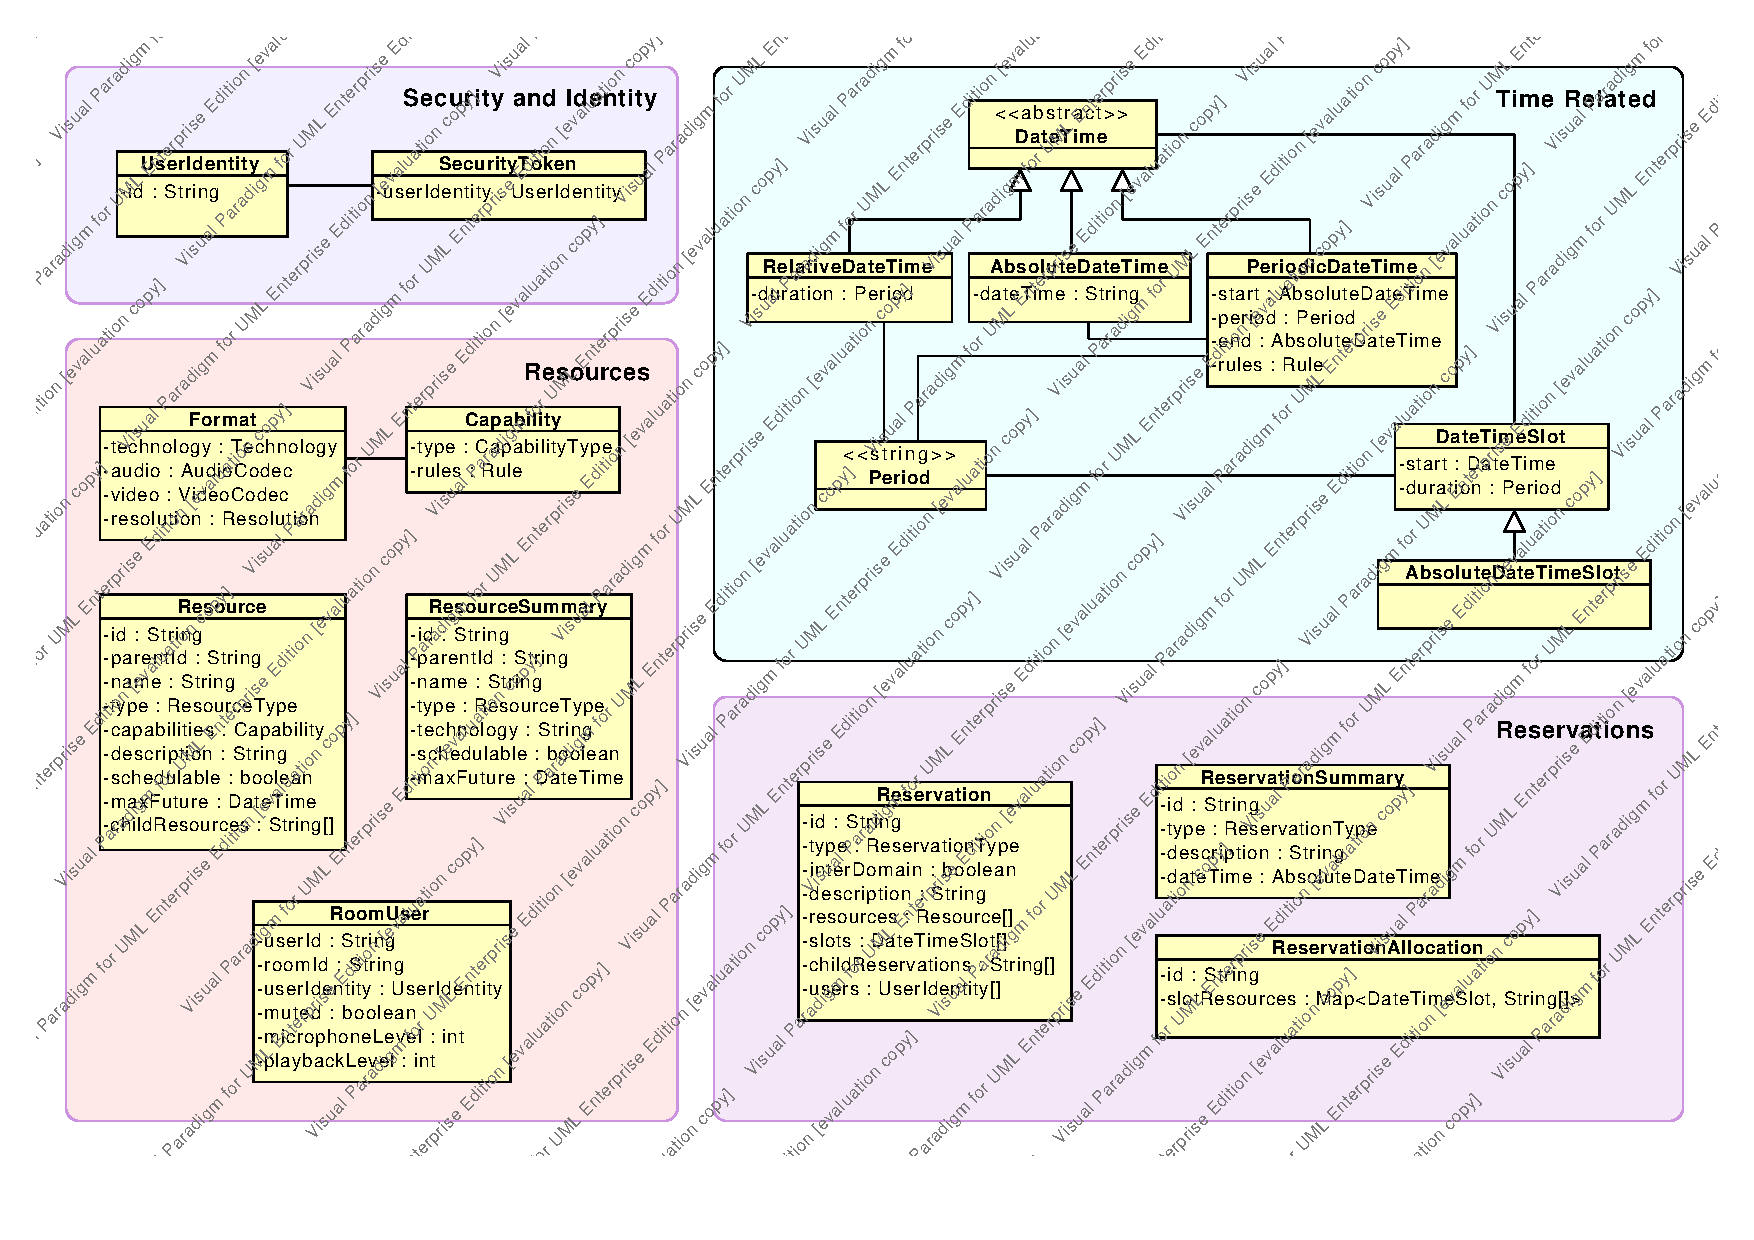
\includegraphics[width=\textwidth]{img/common_data_types.pdf}
\caption{Class Diagram of Common Data Types}
\end{figure}


\chapter{User Interface API Specification}

\section{Data types}

\begin{Api}

\ApiEnum{ControllerType}
Types of controllers in the domain.
\begin{ApiEnumValues}
\ApiEnumValue{Primary}{} The primary controller.
\ApiEnumValue{Backup}{} A backup controller. Behaves just like the primary controller, even some agents may be connected to a backup controller instead of the primary one.
\end{ApiEnumValues}

\ApiClass{ControllerInfo}{}
Represents information about the domain controller.
\begin{ApiClassAttributes}
\ApiClassAttribute{name}{String}{\ApiRequired} A unique name within the domain.
\ApiClassAttribute{description}{String}{\ApiOptional}
\ApiClassAttribute{type}{ControllerType}{\ApiRequired}
\end{ApiClassAttributes}

\ApiClass{Agent}{}
Represents an agent managing a resource.
\begin{ApiClassAttributes}
\ApiClassAttribute{identifier}{String}{\ApiRequired} A unique agent identifier within the domain.
\ApiClassAttribute{address}{String}{\ApiRequired} An address where the agent is reachable.
\ApiClassAttribute{port}{int}{\ApiRequired} Port on which the agent is reachable.
\ApiClassAttribute{resource}{ResourceSummary}{\ApiOptional} Resource managed by the agent.
\end{ApiClassAttributes}

\ApiClass{DomainInfo}{}
Information about a domain and its controller.
\begin{ApiClassAttributes}
\ApiClassAttribute{name}{String}{\ApiRequired} A unique domain name.
\ApiClassAttribute{organization}{String}{\ApiOptional} Organization owning the domain.
\ApiClassAttribute{controller}{ControllerInfo}{\ApiRequired} A controller of the domain.
\ApiClassAttribute{connected}{boolean}{\ApiRequired} Whether a connection to the domain controller is established.
\end{ApiClassAttributes}

\end{Api}

\section{Common}

\begin{Api}

\ApiCmd{ControllerInfo getControllerInfo()}
Get information about the domain controller. See |ControllerInfo| class.

\ApiCmd{Agent[] listAgents(Map filter)}
Lists all agents within the platform (i.e., managed by the controller) managing a resource satisfying a given filter.

\ApiCmd{ControllerInfo[] listControllers()}
Lists the primary and all backup controllers for the domain.

\ApiCmd{DomainInfo[] listDomains()}
Lists all known domains.

\end{Api}


\section{Resources}

\begin{Api}

\ApiCmd{String createResource(SecurityToken token, String domain, Map attributes)}
Create a new resource that will be managed by Shongo. The new resource identifier is returned as a result. The user with given |token| will be the resource owner. Map of |attributes| should contain only attributes specified in |Resource| class and all attributes marked as \ApiRequired\ must be present.

\ApiCmd{modifyResource(SecurityToken token, String resourceId, Map attributes)}
Modify the resource with specified |resourceId|. That operation is permited only when the user with given |token| is the resource owner. Map of |attributes| should contain only attributes specified in |Resource| class.

\ApiCmd{deleteResource(SecurityToken token, String resourceId)}
Delete the resource with specified |resourceId| from Shongo management. That operation is permited only when the user with given |token| is the resource owner and only when the resource is not used in any future reservation.

\ApiCmd{Resource getResource(SecurityToken token, String resourceId)}
Get the complete resource object for specified |resourceId| that a user with given |token| is entitled to see. See |Resource| for details.

\ApiCmd{ResourceSummary[] listResources(SecurityToken token, Map filter)}
List of resources managed by Shongo, that a user with given |token| is entitled to see and that meet the resource |filter| which contains only attributes defined in |ResourceSummary| class. See |ResourceSummary| for details.

\ApiCmd{boolean isResourceActive(SecurityToken token, String resourceId, AbsoluteDateTime dateTime)}
Checks whether the resource with specified |resourceId| is in given |dateTime| used by any reservation.

\ApiCmd{AbsoluteDateTimeSlot[] findResourceAvailableSlots(SecurityToken token, String resourceId)}
Lookup date/time slots when the resource with specified |resourceId| is not allocated to any reservation.


\end{Api}

\subsection{Failures}

\begin{ApiFailures}
\ApiFailure{100}
\end{ApiFailures}
\TODO{Complete this}


\section{Reservations}

\begin{Api}

\ApiCmd{String createReservation(SecurityToken token, ReservationType type, Map attributes)}
Create a new reservation. The new reservation identifier is returned as a result. Map of |attributes| should contain only attributes specified in |Reservation| class and all attributes marked as \ApiRequired\ must be present.

\ApiCmd{modifyReservation(SecurityToken token, String reservationId, Map attributes)}
Modify the reservation with specified |reservationId|. Map of |attributes| should contain only attributes specified in |Reservation| class.

\ApiCmd{deleteReservation(SecurityToken token, String reservationId)}
Release the reservation with specified |reservationId|. The child reservations remain untouched.

\ApiCmd{Reservation getReservation(SecurityToken token, String reservationId)}
Get the reservation object for specified |reservationId| that a user with given |token| is entitled to see. The returned object contains requested time slots, requested resources, child reservations and all other attributes that can be modified. It does not contain the read only scheduler allocation information which can be obtained by |getReservationAllocation|.

\ApiCmd{ReservationAllocation getReservationAllocation(SecurityToken token, String reservationId)}
List all the date/time slots that were allocated by a scheduler for the reservation and for all child reservation (recursive). Each date/time slot contains list of identifiers for resources that are allocated for the date/time slot.

\ApiCmd{ResourceSummary[] listReservationSlotResources(SecurityToken token, String reservationId, AbsoluteDateTimeSlot slot, Map filter)}
Get a list of allocated resources for the given date/time slot in a reservation with specified |reservationId| (one reservation can have multiple date/time slots in which the reservation takes place and the list of allocated resources may vary). The list of resources is filtered by specified |filter| map that should contain only attributes specified in |ResourceSummary|.

\ApiCmd{ReservationSummary[] listReservations(SecurityToken token, Map filter)}
List all the reservations that a user with given |token| is entitled to see and that meet the reservation |filter| which contains only attributes defined in |ReservationSummary| class. Only the lightweight definitions of reservations is returned, see |ReservationSummary| for details.

\ApiCmd{AbsoluteDateTimeSlot[] findReservationAvailableSlots(SecurityToken token, Period duration, Resource[] resources, boolean interDomain)}
Lookup available date/time slots for specified reservation |duration| and |resources|. Argument |interDomain| specifies whether inter-domain lookup should be performed.

\end{Api}

\subsection{Failures}

\begin{ApiFailures}
\ApiFailure{200}
\end{ApiFailures}
\TODO{Complete this}


\section{Room Operations}

\begin{Api}

\ApiCmd{RoomUser[] listRoomUsers(SecurityToken token, String roomId)}
Get the list of users that currently participate in the room with specified |roomId|.

\ApiCmd{RoomUser getRoomUser(SecurityToken token, String roomId, String userId)}
Gets a concrete room user.

\ApiCmd{modifyRoomUser(SecurityToken token, String roomId, String userId, Map attributes)}
Modifies the user with specified |userId| in the room with given |roomId| (suitable for setting microphone/playback level, muting/unmuting\ldots).

\ApiCmd{disconnectRoomUser(SecurityToken token, String roomId, String userId)}
Disconnect the user with specified |userId| from the room with given |roomId|.

\end{Api}

\subsection{Failures}

\begin{ApiFailures}
\ApiFailure{300}
\end{ApiFailures}
\TODO{Complete this}


\chapter{Connector API Specification}

\section{Communication Protocol}

\TODO{Merge with XML-RPC description. Afterwards, just state, what is used for which communication acts (XML-RPC for user interface, Jade ontologies for Jade messaging). Use common failure codes. Groups of failure codes: Shongo-connections, connections between a connector and its device, failures reported by the devices themselves}

Communication among controllers and connectors is implemented using JADE \cite{jade}. The communication is \textbf{synchronous}, i.e., the controller sends a command to a connector and waits until the connector replies. All messages are encoded using the FIPA SL content language \cite{FIPA-SL}. An ontology, called |ShongoOntology|, is used by communicating agents to give the same meaning to the symbols used in messages. This section describes the way commands defined by this API are composed to messages and interpreted by Shongo agents.

The ontology used by all agents consists of concepts, predicates, and agent actions.
\begin{description}
\item[An agent action,] tagged by |jade.content.AgentAction| interface, expresses a request what should the receiving agent do. Each of the commands specified in this API document is defined by a class implementing |AgentAction|, declaring all the command arguments as attributes accessed by public getters and setters.
\item[A predicate,] tagged by |jade.content.Predicate| interface, expresses a claim about a fact. In this API, we use just two predicates defined in the JADE framework, for the purpose of expressing result of a command. We use no custom predicates.
\item[A concept,] tagged by |jade.content.Concept| interface, is any entity which may be a part of an agent action or a predicate. All object types of arguments or return values must be specified as concepts for the agent content manager to be able to properly encode them in messages. In particular, any such a class must implement the |jade.content.Concept| interface and reside within the |cz.cesnet.shongo.ontology| package for the |ShongoOntology| class to be able to find it and comprise it in the ontology used for encoding messages.
\end{description}


For example, the |setMicrophoneLevel(int level)| command, defined in section \ref{sect:connector-endpoint-api}, might be specified by the following class:
\begin{verbatim}
package cz.cesnet.shongo.ontology;

public class SetMicrophoneLevel implements AgentAction {
    private int level = 0;

    public int getLevel() {
        return level;
    }
    public void setLevel(int level) {
        this.level = level;
    }
}
\end{verbatim}
The |setMicrophoneLevel| call implementation instantiates a new |SetMicrophoneLevel| object, sets up the |level| attribute, and passes the object to a controller agent content manager to send it to an endpoint as a |request| communicative act \cite{FIPA-ComActSpec}. The corresponding endpoint agent creates the |SetMicrophoneLevel| object received from the controller agent and implements the requested functionality according to it. The message sent during such a call might be similar to the following:
\begin{verbatim}
(REQUEST
 :receiver  (set ( agent-identifier :name dev@127.0.0.1:1099/JADE ) )
 :content  "((action (agent-identifier :name
     Controller-Main-Container@127.0.0.1:1099/JADE :addresses (sequence
     http://localhost:7778/acc)) (SET-MICROPHONE-LEVEL :level 46)))"
 :language  fipa-sl  :ontology  shongo-ontology )
\end{verbatim}

The agent receiving a command should always send a reply as an |inform| \cite{FIPA-ComActSpec} message. In case of commands without any return value, a |Done| predicate from the package |jade.content.onto.basic| should be sent as a reply, denoting a successful command execution. When a return value is expected, a |Result| predicate, defined in \cite{FIPA-SL}, is sent, filled with the value to be returned. The same requirements apply to the class of the object to be returned as for command object arguments -- the class must reside within the |cz.cesnet.shongo.ontology| interface and be tagged by the |Concept| interface.

An example of a complex command is shown in appendix \ref{appendix:jade-command-encoding}.




\section{Data Types}

\begin{Api}

\ApiClass{ConnectorInfo}{}
Information about connector.
\begin{ApiClassAttributes}
\ApiClassAttribute{name}{String}{} the connector name
\ApiClassAttribute{device}{Resource}{} the device managed by this connector (must be a resource of type ManagedDevice -- see chapter \ref{sect:common:reservations-resources})
\ApiClassAttribute{connectionState}{ConnectionState}{} connection state to the device
\ApiClassAttribute{deviceState}{DeviceState}{} state of the device, maintained by the connector for performance reasons
\end{ApiClassAttributes}

\ApiEnum{ConnectionState}
State of connection between a connector and a device it manages.
\begin{ApiEnumValues}
\ApiEnumValue{Connected}{}
\ApiEnumValue{Disconnected}{}
\end{ApiEnumValues}

\ApiClass{DeviceState}{}
State description of a device.
\TODO{}

\ApiClass{DeviceLoadInfo}{}
Current device load information. A negative value in any attribute means the value could not be determined.
\begin{ApiClassAttributes}
\ApiClassAttribute{cpuLoad}{float}{}
\ApiClassAttribute{memoryOccupied}{long}{}
\ApiClassAttribute{memoryAvailable}{long}{}
\ApiClassAttribute{diskSpaceOccupied}{long}{}
\ApiClassAttribute{diskSpaceAvailable}{long}{}
\end{ApiClassAttributes}

\ApiClass{Room}{}
Represents a virtual room on a multipoint server device.
\begin{ApiClassAttributes}
\ApiClassAttribute{users}{RoomUser[]}{\ApiRequired} List of allowed users.
\ApiClassAttribute{allowGuests}{boolean}{\ApiRequired} A flag indicating whether to allow guest users to join the room.
\ApiClassAttribute{licenseCount}{int}{\ApiRequired} Number of licenses that multipoint server can utilize for this room.
\ApiClassAttribute{layout}{RoomLayout}{\ApiRequired} The default room layout (used for all participants who did not specify a layout of their own choice).
\ApiClassAttribute{configuration}{String[]}{\ApiOptional} Platform specific configuration.
\end{ApiClassAttributes}
\TODO{Room settings should be auto-modified in time be uploaded calendar}

\ApiClass{UsageStats}{}
Usage stats of a given multipoint device.
\begin{ApiClassAttributes}
\ApiClassAttribute{callLog}{byte[]}{} Call log in CDR. Should contain at least start time and duration of each call.
\end{ApiClassAttributes}

\ApiClass{RoomInfo}{}
A brief info about a virtual room at a server.
\begin{ApiClassAttributes}
\ApiClassAttribute{name}{String}{\ApiRequired} Name of the room.
\ApiClassAttribute{owner}{String}{} Identification of the room owner.
\ApiClassAttribute{creation}{AbsoluteDateTime}{} Date and time when the room was created.
\ApiClassAttribute{reservation}{Reservation}{} Reservation for which this room was created (to satisfy use-case \ref{UC:ops:room:shongo-options}).
\ApiClassAttribute{type}{Technology}{} Type of the room.
\end{ApiClassAttributes}

\ApiEnum{RoomLayout}{}
Layout of a virtual room.
\begin{ApiEnumValues}
\ApiEnumValue{SingleParticipant}{only a single, fixed participant is displayed}
\ApiEnumValue{VoiceSwitchedSingleParticipant}{only a single, currently speaking participant is displayed}
\ApiEnumValue{SpeakerCorner}{a fixed participant is in the upper-left corner, other participants around}
\ApiEnumValue{VoiceSwitchedSpeakerCorner}{the currently speaking participant is in the upper-left corner, other participants around}
\ApiEnumValue{Grid}{all participants are spread in a regular grid}
\end{ApiEnumValues}

\ApiClass{MediaData}{}
Custom media data, typically used for uploading or downloading some content (images, documents, etc.).
\begin{ApiClassAttributes}
\ApiClassAttribute{contentType}{ContentType}{\ApiRequired} Type of the data.
\ApiClassAttribute{data}{byte[]}{\ApiRequired} The content. To be interpreted according to the content type.
\ApiClassAttribute{compression}{CompressionAlgorithm}{\ApiOptional} Algorithm used to compress |data|.
\end{ApiClassAttributes}

\ApiClass{ContentType}{}
Description of a media type. Any MIME Media Type listed by IANA \cite{IANA-MediaTypes}, e.g. \texttt{image/jpeg}.
\begin{ApiClassAttributes}
\ApiClassAttribute{type}{String}{\ApiRequired} Textual name of the type (e.g., |image| or |text|).
\ApiClassAttribute{subtype}{String}{\ApiRequired} Textual name of the subtype (e.g., |jpeg| or |html|).
\end{ApiClassAttributes}

\ApiEnum{CompressionAlgorithm}{}
A compression algorithm used to compress data files.
\begin{ApiEnumValues}
\ApiEnumValue{ZIP}{zip compression, as specified by the \texttt{application/zip} MIME type}
\ApiEnumValue{RAR}{rar archive}
\ApiEnumValue{TAR_GZIP}{a gzip-compressed tar archive}
\ApiEnumValue{TAR_BZIP2}{a bzip2-compressed tar archive}
\end{ApiEnumValues}


\end{Api}


\section{Common API}

\begin{Api}

\ApiCmd{ConnectorInfo getConnectorInfo()}
Get information about connector.

\ApiCmd{muteRoomUser(SecurityToken token, String RoomUserId)}
Mutes a user in a room.

\ApiCmd{unmuteRoomUser(SecurityToken token, String RoomUserId)}
Unmutes a user in a room.

\ApiCmd{setMicrophoneLevel(SecurityToken token, String RoomUserId, int level)}
Sets microphone audio level of a user in a room to a given value. Note that the implementation differs between multipoint and endpoint types of devices. On an endpoint, the playback level is set using the device amplifier, while calling this on a multipoint device results in software adaptation of the output sound data (which may result in a distorted sound).

\ApiCmd{setPlaybackLevel(SecurityToken token, String RoomUserId, int level)}
Sets playback audio level of a user in a room to a given value. Note that the implementation differs between multipoint and endpoint types of devices. On an endpoint, the playback level is set using the device amplifier, while calling this on a multipoint device results in software adaptation of the output sound data (which may result in a distorted sound).

\ApiCmd{enableUserVideo(SecurityToken token, String RoomUserId)}
Enables video from a user in a room.

\ApiCmd{disableUserVideo(SecurityToken token, String RoomUserId)}
Disables video from a user in a room.

\end{Api}

\section{Multipoint Device} \label{sect:connector-api-multipoint}

\subsection{Room Management}
\begin{Api}

\ApiCmd{RoomInfo getRoomInfo(SecurityToken token, String roomId)}
Gets info about an existing room.

\ApiCmd{String createRoom(SecurityToken token, Room room)}
Create a new virtual room on a multipoint device that is managed by this connector. The |room| parameter specifies the room settings, see the |Room| definition. Returns an identifier of the created room, unique within the device, to be used for further identification of the room as the |roomId| parameter.

\ApiCmd{modifyRoom(SecurityToken token, String roomId, Map attributes)}
Modifies a room identified by |roomId|. The |attributes| map specifies |Room| attribute names mapped to new values.

\ApiCmd{deleteRoom(SecurityToken token, String roomId)}
Delete an existing virtual room on a multipoint device that is managed by this connector.

\ApiCmd{String exportRoomSettings(SecurityToken token, String RoomId)}
Gets current settings of a room exported to XML.
\\\TODO{Specify schema of the exported XML document in RelaxNG. It should contain at least room name, technology (H.323/SIP/Connect\ldots) settings, and version of the format of the exported document (for further extensions).}

\ApiCmd{importRoomSettings(SecurityToken token, String RoomId, String settings)}
Sets up a room according to given |settings| previously exported by the |exportRoomSettings| method.

\end{Api}


\subsection{User Management}
\begin{Api}

\ApiCmd{RoomUser[] listRoomUsers(SecurityToken token, String roomId)}

\ApiCmd{RoomUser getRoomUser(SecurityToken token, String roomId, String roomUserId)}
Gets user information and settings in a room.

\ApiCmd{modifyRoomUser(SecurityToken token, String roomId, String roomUserId, Map attributes)}
Modifies user settings in the room (suitable for setting
microphone/playback level, muting/unmuting, user layout\ldots).

\ApiCmd{disconnectRoomUser(SecurityToken token, String roomId, String roomUserId)}
Disconnect user from the room.

\ApiCmd{enableContentProvider(SecurityToken token, String roomUserId)}
Enables a given room user as a content provider in the room. This is typically enabled by default.

\ApiCmd{disableContentProvider(SecurityToken token, String roomUserId)}
Disables a given room user as a content provider in the room. Typically, all users are allowed to fight for being the content provider. Using this method, a user is not allowed to do this.

\end{Api}


\subsection{Room Content Management}
\begin{Api}

\ApiCmd{MediaData getRoomContent(SecurityToken token, String roomId)}
Gets all room content (e.g., documents, notes, polls, etc.) as a single archive (see the |compression| attribute of the returned object).

\ApiCmd{addRoomContent(SecurityToken token, String roomId, String name, MediaData data)}
Adds a data file to room content under a given name.

\ApiCmd{removeRoomContentFile(SecurityToken token, String roomId, String name)}
Removes a file of a given name from room content.

\ApiCmd{clearRoomContent(SecurityToken token, String roomId)}
Clears all room content.

\end{Api}


\subsection{Monitoring}
\begin{Api}

\ApiCmd{DeviceLoadInfo getDeviceLoadInfo()}
Gets info about current load of the device.

\ApiCmd{UsageStats getUsageStats()}
Gets the multipoint usage stats.

\ApiCmd{RoomInfo[] getRoomList()}
Gets a list of all rooms at a given server.

\ApiCmd{MediaData getReceivedVideoSnapshot(SecurityToken token, String RoomUserId)}
Gets a snapshot of the video stream received by a user in a room. See the |contentType| of the returned object to get the image format returned.

\ApiCmd{MediaData getSentVideoSnapshot(SecurityToken token, String RoomUserId)}
Gets a snapshot of the video stream that a user is sending in a room. See the |contentType| of the returned object to get the image format returned.

\end{Api}


\subsection{Recording}
\begin{Api}

\ApiCmd{int startRecording(SecurityToken token, String roomId, ContentType format, RoomLayout layout)}
Immediately starts recording in a room to format |format| using a given |layout| (or the default room layout, if |layout| is not specified). Returns an identifier for further reference, unique among other recordings on the device. Does not have any effect and returns 0 if the room is already being recorded.

\ApiCmd{stopRecording(SecurityToken token, int recordingId)}
Stops recording. The |recordingId| parameter, specifying what to stop, is an identifier previously returned by |startRecording| or |scheduleRecording|.

\ApiCmd{String getRecordingDownloadURL(SecurityToken token, int recordingId)}
Returns a URL from where it is possible to download a recording. The |recordingId| parameter is an identifier previously returned by |startRecording| or |scheduleRecording|.

\ApiCmd{notifyParticipants(SecurityToken token, int recordingId)}
Sends an e-mail to all non-anonymous participants present in the room recorded. Participants present in any moment of the recording must be notified, not just the registered users.

\ApiCmd{downloadRecording(SecurityToken token, String downloadURL, String targetPath)}
Starts downloading a recording from |downloadURL|. The recording is stored on the server under |targetPath|.

\ApiCmd{deleteRecording(SecurityToken token, int recordingId)}
Deletes a given recording. The |recordingId| parameter is an identifier previously returned by |startRecording| or |scheduleRecording|. If the recording is being worked with somehow (still being recorded, being uploaded, etc.), the operation is deferred to the moment when current operations are completed.

\end{Api}


\section{Endpoint Device} \label{sect:connector-endpoint-api}

\begin{Api}

\ApiCmd{dial(SecurityToken token, String server)}
Dials a server.

\ApiCmd{resetDevice(SecurityToken token)}
Resets the device.

\end{Api}


\section{Technology Specific API}
\TODO{Cover use cases \ref{UC:ops:room:room-techspec} and \ref{UC:ops:room:user-techspec}.}
\\\TODO{How to structure this section? List the supported commands for each technology separately, or list them on a single place, stating the technologies supporting a functionality for each command?}

\begin{Api}

\ApiCmd{dial(SecurityToken token, String deviceAddress)}
Dials a device, multipoint or endpoint. Dialing a client is available only on \textbf{H.323} and \textbf{SIP}.

\end{Api}


\chapter{Inter-Controller API Specification}


\appendix

\chapter{User Interface API Usage}

\section{Perl programming language}
\newenvironment{PerlCmd}{\small\verbatim}{\endverbatim}
\newenvironment{PerlResponse}{\textbf{Response}\small\verbatim}{\endverbatim}

\subsection{Connect to Controller}

\begin{PerlCmd}
#!/usr/bin/perl

require RPC::XML;
require RPC::XML::Client;

$client = RPC::XML::Client->new('http://localhost:8008');

$response = $client->send_request(...);

if ( ref($response) ) {
    use XML::Twig;
    $xml = XML::Twig->new(pretty_print => 'indented');
    $xml->parse($response->as_string());
    $xml->print();
} else {
    print($response . "\n");
}
\end{PerlCmd}

\newpage
\subsection{Create reservation}
\begin{PerlCmd}
$response = $client->send_request(
    'Reservations.createReservation',
    RPC::XML::struct->new(
        'class' => RPC::XML::string->new('SecurityToken'),
        ...
    ),
    RPC::XML::string->new('OneTime'),
    RPC::XML::struct->new(
        'date' => RPC::XML::struct->new(
            'class' => RPC::XML::string->new('Date'),
            'date' => RPC::XML::string->new('20120101')
        )
    )
);
\end{PerlCmd}
\begin{PerlResponse}
<struct>
  <member>
    <name>class</name>
    <value><string>Reservation</string></value>
  </member>
  <member>
    <name>id</name>
    <value>
      <string>e5a6ee96-8ac5-46dc-ac3b-5374076aee1b</string>
    </value>
  </member>
  <member>
    <name>type</name>
    <value><string>OneTime</string></value>
  </member>
  <member>
    <name>date</name>
    <value><struct>
        <member>
          <name>class</name>
          <value><string>Date</string></value>
        </member>
        <member>
          <name>date</name>
          <value><string>20120101</string></value>
        </member>
    </struct></value>
  </member>
</struct>
\end{PerlResponse}

\newpage
\subsection{Modify reservation}
\begin{PerlCmd}
$response = $client->send_request(
    'Reservations.modifyReservation',
    RPC::XML::struct->new(
        'class' => RPC::XML::string->new('SecurityToken'),
        ...
    ),
    RPC::XML::string->new('15082783-5b6f-4287-9015-3dbc0ab2f0d9'),
    RPC::XML::struct->new(
        'description' => RPC::XML::struct->new() # set description to null
    )
);
\end{PerlCmd}
\begin{PerlResponse}
<struct>
  <member>
    <name>id</name>
    <value><string>15082783-5b6f-4287-9015-3dbc0ab2f0d9</string></value>
  </member>
  <member>
    <name>class</name>
    <value><string>Reservation</string></value>
  </member>
  <member>
    <name>type</name>
    <value><string>OneTime</string></value>
  </member>
</struct>
\end{PerlResponse}

\newpage
\subsection{List reservations}
\begin{PerlCmd}
$response = $client->send_request(
    'Reservations.listReservations',
    RPC::XML::struct->new(
        'class' => RPC::XML::string->new('SecurityToken'),
        ...
    )
);
\end{PerlCmd}
\begin{PerlResponse}
<array><data>
  <value><struct>
    <member>
      <name>class</name>
      <value><string>Reservation</string></value>
    </member>
    <member>
      <name>id</name>
      <value><string>15082783-5b6f-4287-9015-3dbc0ab2f0d9</string></value>
    </member>
    <member>
      <name>type</name>
      <value><string>Periodic</string></value>
    </member>
  </struct></value>
</data></array>
\end{PerlResponse}

\newpage
\subsection{Exception handling}
\subsubsection{Wrong class}
\begin{PerlCmd}
$response = $client->send_request(
    'Reservations.listReservations',
    RPC::XML::struct->new(
        'class' => RPC::XML::string->new('SecurityTokenX'),
        ...
    )
);
\end{PerlCmd}
\begin{PerlResponse}
<fault>
  <value><struct>
    <member>
      <name>faultString</name>
      <value><string>Class 'SecurityTokenX' is not defined.</string></value>
    </member>
    <member>
      <name>faultCode</name>
      <value><i4>1</i4></value>
    </member>
  </struct></value>
</fault>
\end{PerlResponse}

\subsubsection{Wrong attribute name}
\begin{PerlCmd}
$response = $client->send_request(
    'Reservations.listReservations',
    RPC::XML::struct->new(
        'class' => RPC::XML::string->new('SecurityToken'),
        ...
    ),
    RPC::XML::struct->new(
        'typeX' => RPC::XML::string->new('OneTime')
    )
);
\end{PerlCmd}
\begin{PerlResponse}
<fault>
  <value><struct>
    <member>
      <name>faultString</name>
      <value><string>Attribute 'typeX' in class 'Reservation' is not defined.</string></value>
    </member>
    <member>
      <name>faultCode</name>
      <value><i4>2</i4></value>
    </member>
  </struct></value>
</fault>
\end{PerlResponse}

\subsubsection{Wrong attribute value}
\begin{PerlCmd}
$response = $client->send_request(
    'Reservations.listReservations',
    RPC::XML::struct->new(
        'class' => RPC::XML::string->new('SecurityToken'),
        ...
    ),
    RPC::XML::struct->new(
        'type' => RPC::XML::struct->new(
            'class' => RPC::XML::string->new('Date'),
            'date' => RPC::XML::string->new('20120101')
        )
    )
);
\end{PerlCmd}
\begin{PerlResponse}
<fault>
  <value><struct>
    <member>
      <name>faultString</name>
      <value><string>Attribute 'type' in class 'Reservation' has type
          'ReservationType' but 'Date' was presented.</string></value>
    </member>
    <member>
      <name>faultCode</name>
      <value><i4>3</i4></value>
    </member>
  </struct></value>
</fault>
\end{PerlResponse}

\subsubsection{Wrong enum}
\begin{PerlCmd}
$response = $client->send_request(
    'Reservations.listReservations',
    RPC::XML::struct->new(
        'class' => RPC::XML::string->new('SecurityToken'),
        ...
    ),
    RPC::XML::struct->new(
        'type' => RPC::XML::string->new('OneTimeX')
    )
);
\end{PerlCmd}
\begin{PerlResponse}
<fault>
  <value><struct>
    <member>
      <name>faultString</name>
      <value><string>Enum value 'OneTimeX' is not defined in enum
          'ReservationType'.</string></value>
    </member>
    <member>
      <name>faultCode</name>
      <value><i4>4</i4></value>
    </member>
  </struct></value>
</fault>
\end{PerlResponse}

\subsubsection{Bussiness logic exception}
\begin{PerlCmd}
$response = $client->send_request(
    'Reservations.createReservation',
    RPC::XML::struct->new(
        'class' => RPC::XML::string->new('SecurityToken'),
        ...
    ),
    RPC::XML::struct->new(
        'type' => RPC::XML::string->new('Periodic'),
        'date' => RPC::XML::struct->new(
            'class' => RPC::XML::string->new('Date'),
            'date' => RPC::XML::string->new('20120101')
        )
    )
);
\end{PerlCmd}
\begin{PerlResponse}
<fault>
  <value><struct>
    <member>
      <name>faultString</name>
      <value><string>Periodic date is required.</string></value>
    </member>
    <member>
      <name>faultCode</name>
      <value><i4>102</i4></value>
    </member>
  </struct></value>
</fault>
\end{PerlResponse}

\chapter{JADE Command Encoding Example} \label{appendix:jade-command-encoding}

Consider the following command required by this API:
\begin{Api}
\ApiCmd{RoomUser[] listRoomUsers(SecurityToken token, String roomId)}
\end{Api}

The following classes should be defined to represent the command and all objects used by it:
\begin{verbatim}
package cz.cesnet.shongo.ontology;

public class ListRoomUsers implements AgentAction {
    private SecurityToken token;
    private String roomId;

    public String getRoomId() {
        return roomId;
    }
    public void setRoomId(String roomId) {
        this.roomId = roomId;
    }
    public String getToken() {
        return token;
    }
    public void setToken(String token) {
        this.token = token;
    }
}

public class SecurityToken implements Concept {
    private UserIdentity user;

    public UserIdentity getUser() {
        return user;
    }
    public void setUser(UserIdentity user) {
        this.user = user;
    }
}

public class UserIdentity implements Concept {
    private String id;

    public String getId() {
        return id;
    }
    public void setId(String id) {
        this.id = id;
    }
}

public class RoomUser implements Concept {
    private String userId;
    private String roomId;
    private UserIdentity userIdentity;
    private boolean muted;
    private int microphoneLevel;
    private int playbackLevel;

    // getters and setters ...
}
\end{verbatim}

The command might be encoded in the following message:
\begin{verbatim}
(REQUEST
 :receiver  (set ( agent-identifier :name dev@127.0.0.1:1099/JADE ) )
 :content  "((action (agent-identifier :name
     Controller-Main-Container@127.0.0.1:1099/JADE :addresses
     (sequence http://localhost:7778/acc)) (ListRoomUsers)))"
 :language  fipa-sl  :ontology  shongo-ontology )
\end{verbatim}

A successful reply would then be encoded as follows:
\begin{verbatim}
(INFORM
 :sender  ( agent-identifier :name dev@127.0.0.1:1099/JADE  :addresses (sequence
     http://localhost:7778/acc ))
 :receiver  (set ( agent-identifier :name Controller-Main-Container@127.0.0.1:1099/JADE
     :addresses (sequence http://localhost:7778/acc )) )
 :content  "((result (action (agent-identifier :name
     Controller-Main-Container@127.0.0.1:1099/JADE :addresses (sequence
     http://localhost:7778/acc)) (ListRoomUsers)) (sequence (RoomUser :microphoneLevel 45
     :muted false :playbackLevel 0 :roomId konf :userId Azurit :userIdentity
     (UserIdentity :id shongololo)) (RoomUser :microphoneLevel 57 :muted false
     :playbackLevel 0 :roomId konf :userId Shongololo :userIdentity (UserIdentity)))))"
 :reply-with  Controller-Main-Container@127.0.0.1:1099/JADE1336527079398  :language
     fipa-sl  :ontology  shongo-ontology )
\end{verbatim}




\bibliographystyle{elsarticle-num}
\bibliography{IEEEabrv,API}

\end{document}

